\documentclass[11pt,a4paper]{article}
\usepackage[a4paper, total={6in, 9in}]{geometry}
\usepackage[utf8]{inputenc}
\usepackage{tabularx}
\usepackage{enumitem}
\usepackage{microtype}
\usepackage{url}
\usepackage[backend=bibtex8,sorting=none]{biblatex}
\usepackage{pdfpages}
\usepackage{listings}
\usepackage{color}
\usepackage{tikz}
\usepackage[hidelinks]{hyperref}
\usepackage{titlesec}

% set up syntax highlighting for listings
\definecolor{lightgray}{rgb}{.97,.97,.97}
\definecolor{darkgray}{rgb}{.4,.4,.4}
\definecolor{purple}{rgb}{0.65, 0.12, 0.82}
\lstdefinelanguage{JavaScript}{
  keywords=[1]{typeof, new, true, false, catch, function, return, null, catch, switch, var, if, in, while, do, else, case, break, const, let, await, async},
  keywordstyle=[1]\color{blue}\bfseries,
  keywords=[2]{String, Integer},
  keywordstyle=[2]\color{blue}\bfseries,
  ndkeywords={class, export, boolean, throw, implements, import, this},
  ndkeywordstyle=\color{darkgray}\bfseries,
  identifierstyle=\color{black},
  sensitive=false,
  comment=[l]{//},
  morecomment=[s]{/*}{*/},
  commentstyle=\color{purple}\ttfamily,
  stringstyle=\color{red}\ttfamily,
  morestring=[b]',
  morestring=[b]"
}
\lstdefinelanguage{Solidity}{
	keywords=[1]{anonymous, assembly, assert, balance, break, call, callcode, case, catch, class, constant, continue, contract, debugger, default, delegatecall, delete, do, else, event, export, external, false, finally, for, function, gas, if, implements, import, in, indexed, instanceof, interface, internal, is, length, library, log0, log1, log2, log3, log4, memory, modifier, new, payable, pragma, private, protected, public, pure, push, require, return, returns, revert, selfdestruct, send, storage, struct, suicide, super, switch, then, this, throw, transfer, true, try, typeof, using, value, view, while, with, addmod, ecrecover, keccak256, mulmod, ripemd160, sha256, sha3}, % generic keywords including crypto operations
	keywordstyle=[1]\color{blue}\bfseries,
	keywords=[2]{address, bool, byte, bytes, bytes1, bytes2, bytes3, bytes4, bytes5, bytes6, bytes7, bytes8, bytes9, bytes10, bytes11, bytes12, bytes13, bytes14, bytes15, bytes16, bytes17, bytes18, bytes19, bytes20, bytes21, bytes22, bytes23, bytes24, bytes25, bytes26, bytes27, bytes28, bytes29, bytes30, bytes31, bytes32, enum, int, int8, int16, int24, int32, int40, int48, int56, int64, int72, int80, int88, int96, int104, int112, int120, int128, int136, int144, int152, int160, int168, int176, int184, int192, int200, int208, int216, int224, int232, int240, int248, int256, mapping, string, uint, uint8, uint16, uint24, uint32, uint40, uint48, uint56, uint64, uint72, uint80, uint88, uint96, uint104, uint112, uint120, uint128, uint136, uint144, uint152, uint160, uint168, uint176, uint184, uint192, uint200, uint208, uint216, uint224, uint232, uint240, uint248, uint256, var, void, ether, finney, szabo, wei, days, hours, minutes, seconds, weeks, years},	% types; money and time units
	keywordstyle=[2]\color{teal}\bfseries,
	keywords=[3]{block, blockhash, coinbase, difficulty, gaslimit, number, timestamp, msg, data, gas, sender, sig, value, now, tx, gasprice, origin},	% environment variables
	keywordstyle=[3]\color{violet}\bfseries,
	identifierstyle=\color{black},
	sensitive=false,
	comment=[l]{//},
	morecomment=[s]{/*}{*/},
	commentstyle=\color{gray}\ttfamily,
	stringstyle=\color{red}\ttfamily,
	morestring=[b]',
	morestring=[b]"
}
\lstset{
	language=JavaScript,
	backgroundcolor=\color{lightgray},
	extendedchars=true,
	basicstyle=\footnotesize\ttfamily,
	showstringspaces=false,
	showspaces=false,
	numbers=left,
	numberstyle=\footnotesize,
	numbersep=9pt,
	tabsize=2,
	breaklines=true,
	showtabs=false,
	captionpos=b
}

% include shapes and arrows for flow charts and set up
\usetikzlibrary{shapes.geometric, arrows}
\tikzstyle{box} = [rectangle, minimum width=3cm, text width=3cm, minimum height=1cm,text centered, draw=black]
\tikzstyle{startstop} = [rectangle, rounded corners, minimum width=3cm, text width=3cm, minimum height=1cm,text centered, draw=black, fill=red!30]
\tikzstyle{io} = [trapezium, trapezium left angle=70, trapezium right angle=110, minimum width=3cm, text width=3cm, minimum height=1cm, text centered, draw=black, fill=blue!30]
\tikzstyle{process} = [rectangle, minimum width=3cm, text width=3cm, minimum height=1cm, text centered, draw=black, fill=orange!30]
\tikzstyle{decision} = [diamond, aspect=1.2, minimum width=3cm, text width=2cm, minimum height=1cm, text centered, draw=black, fill=green!30]
\tikzstyle{arrow} = [thick,->,>=stealth]
\tikzstyle{doublearrow} = [thick,<->,>=stealth]

% add the file containing our references
\addbibresource{main.bib}

\begin{document}

% fancy title page
\begin{titlepage}
	\centering
	
\includegraphics[width=0.4\textwidth]{res/aston-coa.png}\par\vspace{1cm}
	{\scshape\LARGE Aston University\par}
	\vspace{0.5cm}
	{\scshape\large Final Year Project\\Computer Science\par}
	\vspace{2.5cm}
	{\huge\bfseries Taxicoin: A Decentralised Taxi Protocol\par}
	\vspace{1cm}
	{\Large\itshape Scott Street\par}
	\vspace{0.2cm}
	{\large April 2018\par}
\end{titlepage}

\pagebreak

\abstract{Taxicoin is a decentralised taxi protocol, developed with openness and fairness in mind, and built on Ethereum. This dissertation details the background to the problems Taxicoin attempts to solve, as well as an explanation of the Ethereum network. It then describes the protocol itself, how it has been implemented, and what steps have been taken to ensure the security, reliability and effectiveness of the implementation.}

\tableofcontents

\pagebreak

\section{Introduction}

Taxicoin is an attempt at designing and building a protocol for hailing taxis, where the entire system is fully decentralised, with no single authority in control. The motivation behind this is to combat some of the issues found with existing similar traditional applications, such as \textit{Uber} and \textit{Lyft}.

These companies saw a way to improve the taxi industry and, by improving the user experience and ease of ordering a taxi, attracted many users. However, as was the case with existing taxi companies, they still take a significant cut of fares. Coupled with the fact that they attempt to keep fares lower for passengers, the drivers are left with very little earnings.

In contrast, Taxicoin has been design so that the will of riders and drivers self-regulates fares. A driver decides and quotes fares on an individual basis, rather than being instructed as to what fare they should charge. Riders then judge based on quotes from multiple drivers, along with other criteria such as the driver's rating, which quote they choose to accept.

If the rider believes that none of the quotes are fair, or below the cost threshold desired, then they may negotiate the price with individual drivers, until some agreement is met.

\subsection{Benefits of Decentralisation}

In general, decentralised systems are more open. In context, this means that anybody is free to participate -- one of the key precepts of Taxicoin.

Additionally, such systems, if designed well, should be not in the control of any one group of people. If we look at traditional taxi companies, the customers are at the will of the company. In many cases, one company will form the sole taxi coverage of a territory, meaning that they can decide on the price for a journey.

With a decentralised system, decisions about such issues are made transparently between all parties involved. Because information about past fares is available for all to see, this can be used as a benchmark to judge what fares should be for future rides. If drivers quote a fare significantly higher than previous for a similar journey, they should be expected to qualify this decision. This creates a fairer experience for riders, while still allowing drivers to make adjustments under exceptional circumstances.

\subsection{Why an Open Protocol}

Continuing with the themes of decentralisation, it was important that Taxicoin be as open as possible. If a single entity was tasked with developing, maintaining and championing the Taxicoin network, and decided to cease doing so in a scenario where the protocol specification or implementation source code was not openly available, the system would likely stagnate.

It also would create a \textit{walled garden} scenario, where a single entity has total control over the system. They could decide at any point to disregard the original decisions made behind the network, and start charging a fee for each journey. As users are already well invested in using the application, with their reputation accrued significantly, they are likely to continue using it, but now with a less satisfactory experience. They become in a situation where they are at the will of a single entity (as is currently the case with Uber).

But with an open protocol, the specification needed to implement one's own version of Taxicoin is freely available. If users in a certain location beyond that which is actively supported by the initial version wish to launch their own Taxicoin, they can. It also allows for continued critique and improvement, where potential bugs can be discovered and fixed, and if a developer external to the original project wishes to write an extension to the protocol to add further features, they may do so.

\section{An Explanation of Ethereum}

Ethereum is a platform consisting of three components: Swarm, a “distributed storage platform and content distribution service” \cite{Swarm}; Whisper, a peer-to-peer communication protocol \cite{Whisper}; and the Ethereum Virtual Machine (EVM) used for running smart contracts \cite{Ethereum}. The latter is often referred to alone simply as “Ethereum”, however all three should be considered part of the same platform, each one complimenting the others. The aim of this section is to explain how these three solutions are used together to develop fully decentralised applications, or dApps.

\subsection{Blockchains}

The EVM component of Ethereum is built on top of a “blockchain”, a term coined by the anonymous creator of Bitcoin \cite{Bitcoin}, which is the original, and most widely known application of such technology. At its core, a blockchain consists of transactions, grouped together into “blocks”, with each group also referencing the previous one, thus forming a “chain”. A blockchain can be thought of simply as a form of database, keeping a state. A transaction represents a state transition, but must be verified before being deemed to be valid and placed in a block.

% TODO: blockchain diagram here?

The blockchain itself is distributed across all nodes in the network (except in cases where a node chooses to reference another’s copy), meaning that, unless explicitly obfuscated by the user, all transaction data on the network is open. This allows the auditing of transactions by any node on the network, and eliminates the need to trust a single entity to provide accurate data - this is the concept of trustlessness.

Transactions on the Bitcoin blockchain are, for the most part, simply that - transactions. They represent a transfer of funds from one "address" to another. They can additionally contain an amount of data, representing anything from a simple message, to a method call in cases where the receiving address is a “smart contract" (or simply “contract”).

In Bitcoin, contracts are a special type of address which causes nodes on the network to execute some predefined code when a transaction is sent to it. Contracts are deployed by a standard (human controlled) address, but once deployed act as independent entities. Unless their code contains functionality to do so, the deployer has no control over the contract.

However, contract execution on the Bitcoin network is not Turing complete, due to the halting problem - the inability to determine whether a section of code will complete execution without looping infinitely. If contract execution was Turing complete in the existing Bitcoin network, a malicious actor would be able to perform a denial of service attack against the network by deploying and calling contact code containing an infinite loop.

This is where the EVM differs, with the addition of “gas”. This introduces a fee per instruction to be executed (paid in Ethereum’s native cryptocurrency, Ether). The sender of a transaction sets the maximum amount of gas they are willing to spend for a transaction to complete, and a contract call will continue executing until either the execution completes, or the maximum amount of gas is consumed. This safely allows the use of loops within contracts, as it becomes very expensive to perform an infinite-loop attack.

The result is that the EVM is Turing complete, and thus in theory any arbitrary program can be implemented in a contract, opening the door to a wide variety of applications.

\subsection{dApps}

While smart contracts are well suited to taking inputs, making state changes, and producing outputs, that is all they do. It is possible to interact with them via a command line interface, through an Ethereum node, however this is obviously far from the desired experience for end users. To address this problem, several attempts at providing a user interface layer for the Ethereum network have been introduced. The most widely adopted, and officially endorsed solution [cite], is Web3 - a browser API which allows interacting with all parts of the Ethereum platform from Javascript embedded on a web page.

% TODO: cite endorsement

This leads to the approach that many Ethereum dApp developers take: considering their application as a traditional “Single Page App”, where instead of calling HTTP API endpoints, they are now interacting with a smart contract through the use of Web3. Smart contracts effectively take the place of a “backend” web server, leading to many benefits over traditional web apps, such as availability, security and integrity: a single fault in the system does not result in access being denied to users as would be the case with a web server becoming unavailable; there is no need to trust that information will be securely kept on a company's servers, instead strong encryption is used which may be independently audited; and the state of an application is kept by a smart contract whose functionality is publicly available to see and cannot be tampered with - if it is correctly implemented its state cannot be maliciously changed.

Coupling this with Whisper allows for peer-to-peer communication between instances of a dApp, which in most cases translates to between different users. For example, two parties negotiating the price of an item to be purchased - they do not necessarily want their negotiation to be public (or rather, it does not provide any value for it to be), therefore they can come to an agreement “off-chain” before publishing (sending) a transaction of the final agreed price. Whisper is also beneficial for situations where the sender of a message wishes to remain anonymous. When publishing a transaction on the blockchain, the sender is published along with it, whereas in Whisper, unless signed, it is improbable to determine the sender of a message [cite]. % TODO: cite shh plausible deniability

Additionally, the static HTML, Javascript and any additional components of a dApp can be hosted from Swarm (or a similar platform such as IPFS [cite]). When a file, or set of files, is published to Swarm, a hash is computed, and the file is split into pieces called “shards”. The shards are then distributed across nodes in the network, with the intention that if one node becomes unavailable, the shards of the file should still be accessible. When a user wishes to retrieve a file at a later date, they can provide the previously computed hash to a Swarm node, which will request shards of the file from its connected peers. % TODO: cite IPFS

In this manner, it is possible with the Ethereum platform to develop fully decentralised applications where the user interface is written as a web page and is served from Swarm, thus eliminating the requirement for a traditional web server. An application’s “backend” logic is contained within a smart contract, removing the need for a backend web server such as PHP. And finally, instances of the application may communicate between each other through the use of Whisper, removing the need for a solution such as WebSockets, where a central signalling server is required.

\subsection{Solidity Language}

The language most commonly used to develop smart contracts is a domain specific language called Solidity [cite]. It features a C-like syntax, static typing, and supports \enquote{inheritance, libraries and complex user-defined types}. % TODO: cite

While Solidity is still relatively young in comparison with more well-known languages, it is mature enough to use in production environments.

A simple example of a typical contract written in Solidity is as follows:

\begin{lstlisting}[language=Solidity]
contract MyContract {
  // instance variables keep the state of the contract
  uint public counter;

  // constructor is called when the contract is deployed to a network
  constructor() public {
    counter = 0;
  }

  // functions may be defined which perform some action when called
  function increaseCount(uint by) public {
    counter += by;
  }
}
\end{lstlisting}

There are also many more domain-specific features, such as an \lstinline{address} type, representing an address on the network, as well as global variables for accessing the state of the blockchain, and properties of the transaction which is calling the contract.

\subsection{Smart Contract System Design}

As smart contract execution is only ever triggered as a result of a transaction, applications must be designed around deliberate actions. For example, where in a traditional system, a method may be set to execute at a particular date and time, in a smart contract this is not possible. Instead such a method may only have a check for if the allowed time of execution has passed, and must be manually triggered by a transaction.

As the reasons for some of these differences are unlikely to be clear to users, it is important to consider how to communicate them.

Additionally, as there is an attached "gas" fee for publishing transactions and calling contract methods, it is in the interests of the users for the contract developer to make contracts as efficient as possible, and to make a minimal number of contract calls in a dApp. One way of doing this is to avoid on-chain interaction wherever possible, through the use of peer-to-peer protocols, predominantly Whisper. In extreme cases, complex routines within contracts can be written in the underlying EVM byte-code for improved efficiency.

\subsection{Why Ethereum}

There are a multitude of different projects aiming to be a platform for building decentralised applications upon, however none offer such a rich feature set and relative stability as Ethereum does.

The majority of other decentralisation projects are stateless, meaning that between two participants, there must be some kind of storage mechanism if they wish for the data being sent to be kept. In the example of a messaging application, this would mean that each party would need to independently store the message history. If all participants were to lose the history, there would be no way of recovering it. Alternatively a complex infrastructure for message storage could be developed by an application's developers.

Blockchain-based platforms offer a solution where the application developer need not worry about the infrastructure for managing state. And among such solutions, Ethereum is the most appealing, again due to its features, but also the number of users.

Compared with NEO [cite], an alternative blockchain-based platform which supports smart contracts, Ethereum has a much larger development community, and has many more projects being developed with it as the basis. In this new field, it is likely sensible to \enquote{go with the masses}, as from a user perspective, it is a much more pleasant experience to only need to install tools to interact with a single blockchain.

Additionally, from a developer point of view, as more applications are developed on a single blockchain, the interoperability of these allows more and more complex integrations to be built.

\pagebreak
\section{Identification of Requirements}

The first step towards developing Taxicoin was to identify the requirements for the resulting system. These were split into two categories: minimum viable and additional requirements.

\subsection{Minimum Viable Requirements}

These requirements are those which must be included in order for the system to correctly function.

\bigskip\textbf{Drivers must be required to pay a deposit in order to advertise} to act as a reasonable barrier to entry. Without this in place, the network is easily open to spam and scammers posing as drivers. The deposit acts as an incentive to behave well.

\bigskip\textbf{Riders must advertise jobs to drivers on an individual basis} in order to protect the privacy of the rider. As this is likely to contain individually identifying information, such as location, if this were published it could be used to track an individual.

\bigskip\textbf{The fare must be determined by quotes from driver} to remove the need for a centralised fare decision. This is due to the fact that the fare depends on many factors which cannot be automatically determined in a decentralised and reliable manner, such as distance and demand. The alternative would be fixed fares, but this is highly undesirable as short trips would be overpriced, and long trips underpriced.

\bigskip\textbf{Riders must pay fares to a contract in advance} as a security measure, due to the fact that there is no other way to guarantee riders will pay after the fact. Without this, it is likely that a subset of riders would not pay for journeys.

\bigskip\textbf{Riders must provide an additional deposit before starting a journey} to act as an incentive to successfully and formally complete a journey in the system. Without this, riders may have paid fare and have no regard for consequences of bad acts. Additionally, they may not carry on to rate the driver, an integral part of the smooth running of the system.

\bigskip\textbf{Riders and drivers must both rate the other on completion of a journey} to affect the reputation of the other party. This is likely to be implemented such that a user is unable to interact with the rest of the system until they have formally completed their previous journey. Without this requirement, there is no way to determine the trustworthiness of another individual on the network, which is key to preventing bad behaviour.

\bigskip\textbf{When a journey is completed, deposits should be returned to the respective parties, and the fare paid to the driver} this ensures that riders and drivers both have a stake in formally completing a journey. If they do not, their deposits are not returned, and neither is the driver paid. Without this deposit system, there is no guarantee that either party will rate the other - potential hit-and-run scenarios could occur where a rider uses the system only once and does not care to formally complete a journey and rate their driver as it provides no benefit to them. With the deposits however, they are likely to complete the process, at stake of losing their funds.

\subsection{Additional Requirements}

These are requirements deemed as \enquote{nice to have} features, without which the system will continue to function, but the addition of which would improve the system in some way.

\bigskip\textbf{Prospective drivers and riders should be able to informally communicate before forming a contract} to allow any additional requirements on either part be known. For example if a rider is wishing to take a large, bulky item on the journey with them, they may communicate this in advance. If it transpires that the driver's car is small, the journey can be cancelled (or not formally begun), and another driver arranged, before the original driver has taken the effort of travelling to pick up the rider.

\bigskip\textbf{Dispute resolution should be built into the system} for situations where driver and rider are unable to successfully complete a journey. This would work in a similar way to negotiating a price. In a worst case scenario, the driver wants payment in full, but the rider wants to pay nothing. In this case, the two negotiate until an agreement is reached. If they do not reach such an agreement, it reflects poorly on both parties, as the fact that they have an unresolved dispute is public. The system is able to function without this, but bad disputes are likely to go unresolved which is dissatisfactory.

\section{Protocol Specification}

The protocol portion of Taxicoin is designed to be open. As such, anybody should be able to implement it in their own software. The following section of this document should be sufficient to do so.

\subsection{Methods}

Each of these methods is intended to be part of a smart contract. When one is called, it will modify the state of the contract, and/or return a value. Any action taken through a contract is considered to be \textit{formal} and binding (once the other party has agreed where applicable).

The specified arguments are to be supplied when calling that function of the contract, with the types representing built-in Solidity language types. The \textit{payable} keyword indicates that a method accepts a transaction with a currency value attached. In instances where the preconditions for a method are not met, the method will revert and the state will be unmodified.

\subsubsection{Driver Advertise}

\begin{description}[leftmargin=8em,style=nextline]
	\item [Description]
		Takes a deposit from a driver and publishes their location and public key.
	\item [Arguments]
		Latitude: String\footnotemark \\
		Longitude: String \\
		Public Key: String
	\item [Payable]
		Driver deposit
	\item [Preconditions]
		User must not be currently on a journey, either as a driver or rider. Deposit must either have been already provided, or sent with this transaction.
	\item [Postconditions]
		The driver's location and public key are published, and the value of the deposit provided by the driver is recorded. If any deposit over the required amount was provided with the transaction, the excess is returned.
\end{description}

\footnotetext{Strings are used for latitude and longitude as floating point numbers can introduce inaccuracies due to the way they are stored.}

\subsubsection{Driver Advert Revoke}

\begin{description}[leftmargin=8em,style=nextline]
	\item [Description]
		Removes an active driver's advertisement.
	\item [Arguments]
		None
	\item [Payable]
		No
	\item [Preconditions]
		User must be advertised as a driver.
	\item [Postconditions]
		The driver is removed from the list of active drivers, indicating that riders should not send job proposals to this driver. The previously supplied deposit is not returned.
\end{description}

\subsubsection{Rider Create Journey}

\begin{description}[leftmargin=8em,style=nextline]
	\item [Description]
		Accepts a quoted fare for a journey as a rider and forms the rider's part of a contract between driver and rider. Intended to be called after an off-chain negotiation with \lstinline{job} and \lstinline{quot} messages.
	\item [Arguments]
		Driver Address: address \\
		Fare: uint, value in \textit{wei}\footnotemark, $n > 0$ \\
		Public Key: String
	\item [Payable]
		Fare plus rider deposit
	\item [Preconditions]
		The user at the provided address must be an actively advertised driver, and not currently on a journey. The user calling this method must not be an actively advertised driver, nor be part of a journey as either rider or driver. The full rider deposit, plus an amount equal to the provided \lstinline{fare} must have been provided with this transaction.
	\item [Postconditions]
		The rider's intent to travel with the specified driver at the specified price is published. At this stage, the agreement is not binding until the driver accepts, before which the journey may be cancelled, with the rider deposit and fare being returned in full.
\end{description}

\footnotetext{Wei is the smallest denomination of the Ether currency used in the Ethereum network.}

\subsubsection{Rider Cancel Journey}

\begin{description}[leftmargin=8em,style=nextline]
	\item [Description]
		Cancels a journey which has not yet been accepted by a driver.
	\item [Arguments]
		None
	\item [Payable]
		No
	\item [Preconditions]
		Rider must be part of a journey, for which the driver has not already accepted.
	\item [Postconditions]
		The rider is removed from the journey. From this point it is no longer possible for the driver to accept the journey. The rider's deposit and fare are returned.
\end{description}

\subsubsection{Driver Accept Journey}

\begin{description}[leftmargin=8em,style=nextline]
	\item [Description]
		Formally accepts a job as a driver, committing both the rider and driver to its completion.
	\item [Arguments]
		Rider Address: address \\
		Fare: uint, value in \textit{wei} $n > 0$
	\item [Payable] 
		No
	\item [Preconditions]
		Driver must be actively advertised and have provided the driver deposit. Rider must have formally created a journey with the driver set to the caller of this method, and the fare of equal value to the argument provided.
	\item [Postconditions]
		The driver is marked as being on a journey with the specified rider. From this point, the journey is considered to be in progress, and any attempt to change any aspect of the journey will require an agreement to be made between both rider and driver.
\end{description}

\subsubsection{Complete Journey}

\begin{description}[leftmargin=8em,style=nextline]
	\item [Description]
		Marks the current journey as completed, as either the rider or driver.
	\item [Arguments]
		Rating: uint8, $1 \leq n \leq 255$ with 255 being the \enquote{best}
	\item [Payable] No
	\item [Preconditions]
		The caller of the method must either be a driver or rider who is currently on a journey.
	\item [Postconditions]
		The caller of the method is marked as having completed the journey, however they are still part of this journey until the other user has also called this method. The rating for the other user is stored. If the other party has already called this method, then the ratings for both parties are applied to their overall rating, and the journey is formally completed. The rider and driver deposits are returned, and the fare transferred to the driver. However, in cases where the fare is zero (only possible where the fare has been altered during a journey to indicate that the journey should be cancelled), the driver's deposit is not returned.
\end{description}

\subsubsection{Driver Propose Fare Alteration}

\begin{description}[leftmargin=8em,style=nextline]
	\item [Description]
		Formally proposes the alteration of the fare for a journey. Intended to be called after an off-chain negotiation with \lstinline{Propose Fare Alteration} messages.
	\item [Arguments]
		New Fare: uint, value in \textit{wei}
	\item [Payable]
		No
	\item [Preconditions]
		The user calling the method must be a driver, and currently be on a journey.
	\item [Postconditions]
		The driver's proposed new fare is recorded. The new fare does not take effect until the rider calls the \lstinline{Confirm Fare Alteration} method.
\end{description}

\subsubsection{Rider Confirm Fare Alteration}

\begin{description}[leftmargin=8em,style=nextline]
	\item [Description]
		Confirms the alteration of the fare for a journey.
	\item [Arguments]
		New Fare: uint, value in \textit{wei}
	\item [Payable]
		Difference between old and new fares, if new is higher
	\item [Preconditions]
		The user calling the method must be currently on a journey. Driver must have previously agreed the same new fare with the \lstinline{Alter Fare} method. In the case that the new fare is higher, the difference must have been provided with this transaction.
	\item [Postconditions]
		The new value for the fare for the journey is recorded. In the case that the new fare is lower, the difference is returned to the rider. If the new fare is zero, the journey is considered to be cancelled - the journey may now be completed with the rider's deposit being returned, and no fare being paid to the driver.
\end{description}

\subsubsection{Get User Type}

\begin{description}[leftmargin=8em,style=nextline]
	\item [Description]
		Returns an integer representing the type of user at the provided address.
	\item [Arguments]
		User Type: uint8
	\item [Payable]
		No
	\item [Preconditions]
		None
	\item [Postconditions]
		Returns an integer between 0 and 3, representing the enum \{ None, Driver, ActiveDriver, Rider \}.
\end{description}

\subsubsection{Get Driver}

\begin{description}[leftmargin=8em,style=nextline]
	\item [Description]
		Returns the details of the driver at the given address.
	\item [Arguments]
		Driver Address: address
	\item [Payable]
		No
	\item [Preconditions]
		None
	\item [Postconditions]
		If the address provided is of a user who has previously (or is currently) advertised as a driver, the details of the driver will be returned.
		
		Otherwise, all zero-values will be returned.
\end{description}

\subsubsection{Get Next Driver}

\begin{description}[leftmargin=8em,style=nextline]
	\item [Description]
		Returns the details of the driver next in the list of advertised drivers after the given address.
	\item [Arguments]
		Driver Address: address
	\item [Payable]
		No
	\item [Preconditions]
		None
	\item [Postconditions]
		If the address provided is of a user who has previously (or is currently) advertised as a driver, the details of the next driver in the list will be returned.
		
		If the zero-address (\lstinline{0x0}) is provided, the first driver in the list is returned.
		
		If the address provided is for the last driver in the list, the zero-address is returned.
\end{description}

\subsubsection{Get Previous Driver}

\begin{description}[leftmargin=8em,style=nextline]
	\item [Description]
		Returns the details of the driver previous in the list of advertised drivers after the given address.
	\item [Arguments]
		Driver Address: address
	\item [Payable]
		No
	\item [Preconditions]
		None
	\item [Postconditions]
		If the address provided is of a user who has previously (or is currently) advertised as a driver, the details of the previous driver in the list will be returned.
		
		If the zero-address (\lstinline{0x0}) is provided, the last driver in the list is returned.
		
		If the address provided is for the first driver in the list, the zero-address is returned.
\end{description}

\subsubsection{Get Rider}

\begin{description}[leftmargin=8em,style=nextline]
	\item [Description]
		Returns the details of the rider at the given address.
	\item [Arguments]
		Rider Address: address
	\item [Payable]
		No
	\item [Preconditions]
		None
	\item [Postconditions]
		If the address provided is of a user who has previously used (or is currently using) the system as a rider, the details of the rider will be returned.
		
		Otherwise, all zero-values will be returned.
\end{description}

\subsection{Messages}

Driver and rider user clients should be listening for the following messages, where applicable. These messages are communicated via the Whisper protocol.

Message topics are always a length of 4 bytes (4 ASCII characters), therefore any topics listed here of a length less than 4 byes are right-padded with spaces.

\subsubsection{Job Proposal}

\begin{description}[leftmargin=6em,style=nextline]
	\item [Topic]
		\lstinline{job}
	\item [Purpose]
		This message is sent by a rider to a prospective driver, indicating that they wish to make the described journey. It is intended to be sent to advertised drivers matching a specified criteria, e.g. within a certain distance, with at least a certain reputation.
		
		However the sending of these messages is not intended to be carried out manually by the user -- rather there is an automated process which fetches the list of active drivers and determines which to propose to.
	\item [Response]
		Should a driver be interested in a proposal, they respond with a quote message.
	\item [Payload]
		Please see below.
\end{description}

\lstinputlisting{res/job-message.json}

\subsubsection{Driver Quote}

\begin{description}[leftmargin=6em,style=nextline]
	\item [Topic]
		\lstinline{quot}
	\item [Purpose]
		This message is sent by a driver as a response to a job proposal. It contains the network address of the driver, as well as the fare for which the driver is willing to take on the job. At this point, the quote is not binding.
		
		Quote messages with a fare of -1 are considered to be a rejection, indicating that the driver does not wish to accept this job.
	\item [Response]
		If the rider chooses to accept the quote, they next call the create journey method, and respond with a \lstinline{Journey Created} message.
	\item [Payload]
		Please see below.
\end{description}

\lstinputlisting{res/quote-message.json}

\subsubsection{Journey Created}

\begin{description}[leftmargin=6em,style=nextline]
	\item [Topic]
		\lstinline{crea}
	\item [Purpose]
		This message is sent by a rider to a driver after they have created a journey. This is an indication that the rider has accepted the driver's quote.
	\item [Response]
		The driver should next call the \lstinline{Driver Accept Journey} method, and respond with a \lstinline{Journey Accepted} message.
	\item [Payload]
		Please see below.
\end{description}

\lstinputlisting{res/created-message.json}

\subsubsection{Journey Accepted}

\begin{description}[leftmargin=6em,style=nextline]
	\item [Topic]
		\lstinline{accp}
	\item [Purpose]
		This message is sent by a driver to a rider, after they have formally accepted the rider's journey, to indicate that both parties are now on a journey.
	\item [Response]
		None
	\item [Payload]
		Please see below.
\end{description}

\lstinputlisting{res/accepted-message.json}

\subsubsection{Driver Location}

\begin{description}[leftmargin=6em,style=nextline]
	\item [Topic]
		\lstinline{lctn}
	\item [Purpose]
		Sends the location of the driver to the rider with whom they are currently on a journey with. Allows the rider's client to display how far the driver is from the pickup location.
	\item [Response]
		None
	\item [Payload]
		Please see below.
\end{description}

\lstinputlisting{res/location-message.json}

\subsubsection{Journey Completed}

\begin{description}[leftmargin=6em,style=nextline]
	\item [Topic]
		\lstinline{cmpl}
	\item [Purpose]
		This message is sent to the other party when either one calls the \lstinline{Complete Journey} method. It indicates that the other should also (or dispute it). If the other party has already completed the journey, then this message indicates that the journey is fully complete.
	\item [Response]
		None
	\item [Payload]
		None
\end{description}

\subsubsection{Propose Fare Alteration}

\begin{description}[leftmargin=6em,style=nextline]
	\item [Topic]
		\lstinline{nfar}
	\item [Purpose]
		This message is sent to the other party to indicate that the user wishes to alter the fare for the current journey.
	\item [Response]
		If the message is received by a driver for the first time, unprompted, they may either agree with the new proposed fare, and formally propose the new fare with the \lstinline{Propose Fare Alteration} method, or reject the new fare by sending a message of this type with an alternate fare.
		
		If the message is received by a driver for the second time, after agreeing to the proposed new fare, and the value in this message is unchanged, this indicates that the rider has called the \lstinline{Rider Confirm Fare Alteration} method, and the new fare has been applied. No further response is sent. However if the fare was changed, the driver may act as if this is the first such message (see above).
		
		If the message is received by a rider for the first time, unprompted, the rider may either agree to the new fare, and respond with a message of the same type with an unchanged value, or they may disagree and respond with their proposed new fare.
		
		If the message is received by a rider for the second time, after agreeing to the proposed new fare, and the value is unchanged, this indicates that the driver has called the \lstinline{Propose Fare Alteration} method, and that the rider should call the \lstinline{Rider Confirm Fare Alteration} method. They then respond with a message of this type, with the fare value unchanged.
	\item [Payload]
		Please see below.
\end{description}

\lstinputlisting{res/new-fare-message.json}

\subsection{Contract Solidity Interface}

The above methods can be translated to a Solidity interface, which should be conformed to for all Ethereum-based contracts implementing the Taxicoin protocol. This aids the goal of creating an open ecosystem as, in theory, if all implementations conform to this standard, any client should be able to work with any contract implementation.

\lstinputlisting[language=Solidity]{../contracts/ITaxicoin.sol}

\subsection{Protocol Network Architecture}

This diagram is a high-level explanation of how the various components of the Taxicoin protocol fit together.

\begin{figure*}[h!]
\centering
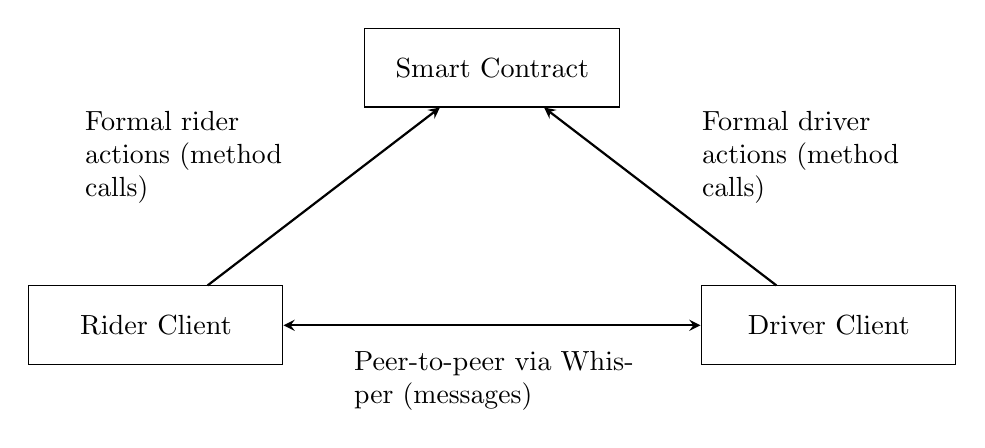
\begin{tikzpicture}[node distance=1.8cm]
	\node (n0) [box] {Smart Contract};
	\node (n1) [box, below left of=n0, yshift=-2cm, xshift=-3cm] {Rider Client};
	\node (n2) [box, below right of=n0, yshift=-2cm, xshift=3cm] {Driver Client};
	
	\draw [arrow] (n1) -- node[anchor=east, text width=2.5cm, above=0.5cm, left=0.4cm] {Formal rider actions (method calls)} (n0);
	\draw [arrow] (n2) -- node[anchor=west, text width=2.5cm, above=0.5cm, right=0.4cm] {Formal driver actions (method calls)} (n0);
	\draw [doublearrow] (n1) -- node[anchor=north, text width=3.5cm, below=0.2cm] {Peer-to-peer via Whisper (messages)}(n2);
\end{tikzpicture}
\end{figure*}

As seen in the above figure, the smart contract acts as an \enquote{orchestrator} of sorts. Informal messages between a rider and driver are first conducted off-chain, as explained previously, and formal binding actions are performed through the contract.

Although this architecture assumes the use of Ethereum smart contracts and the Whisper protocol for sending messages, any infrastructure may be used on which it is possible to implement an application which satisfies the protocol standard. Note that if another platform is used, it will not be interoperable with others based on the assumed technologies.

\pagebreak
\subsection{Process Flow Diagram}

This describes the possible routes of interaction through the system.

\begin{figure*}[h!]
\centering
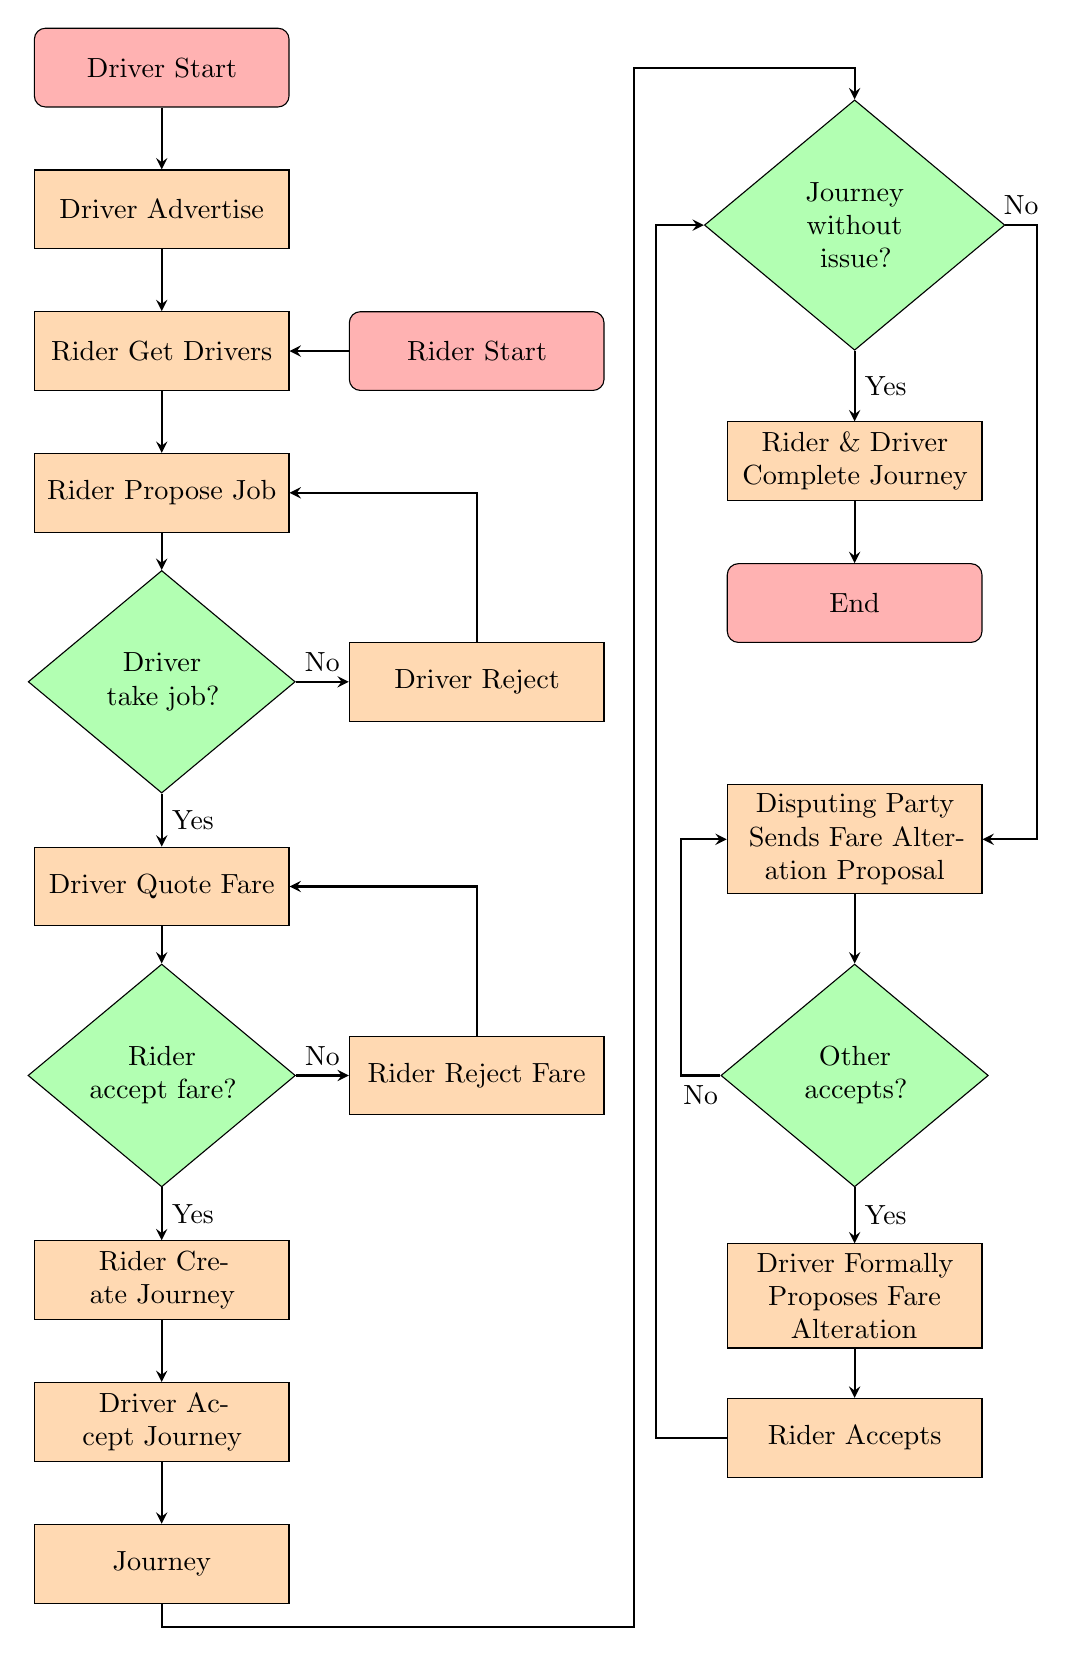
\begin{tikzpicture}[node distance=1.8cm]
	\node (n0) [startstop] {Driver Start};
	\node (n1) [process, below of=n0] {Driver Advertise};
	\node (n2) [process, below of=n1] {Rider Get Drivers};
	\node (n3) [startstop, right of=n2, xshift=2.2cm] {Rider Start};
	\node (n4) [process, below of=n2] {Rider Propose Job};
	\node (n5) [decision, below of=n4, yshift=-0.6cm] {Driver take job?};
	\node (n6) [process, right of=n5, xshift=2.2cm] {Driver Reject};
	\node (n7) [process, below of=n5, yshift=-0.8cm] {Driver Quote Fare};
	\node (n8) [decision, below of=n7, yshift=-0.6cm] {Rider accept fare?};
	\node (n9) [process, right of=n8, xshift=2.2cm] {Rider Reject Fare};
	\node (n10) [process, below of=n8, yshift=-0.8cm] {Rider Create Journey};
	\node (n11) [process, below of=n10] {Driver Accept Journey};
	\node (n12) [process, below of=n11] {Journey};
	\node (n13) [decision, right of=n0, xshift=7cm, yshift=-2cm] {Journey without issue?};
	\node (n14) [process, below of=n13, yshift=-1.2cm] {Rider \& Driver Complete Journey};
	\node (n15) [startstop, below of=n14] {End};
	\node (n16) [process, below of=n15, yshift=-1.2cm] {Disputing Party Sends Fare Alteration Proposal};
	\node (n17) [decision, below of=n16, yshift=-1.2cm] {Other accepts?};
	\node (n18) [process, below of=n17, yshift=-1cm] {Driver Formally Proposes Fare Alteration};
	\node (n19) [process, below of=n18] {Rider Accepts};
	
	\draw [arrow] (n0) -- (n1);
	\draw [arrow] (n1) -- (n2);
	\draw [arrow] (n3) -- (n2);
	\draw [arrow] (n2) -- (n4);
	\draw [arrow] (n4) -- (n5);
	\draw [arrow] (n5) -- node[anchor=south] {No} (n6);
	\draw [arrow] (n6) |- (n4);
	\draw [arrow] (n5) -- node[anchor=west] {Yes} (n7);
	\draw [arrow] (n7) -- (n8);
	\draw [arrow] (n8) -- node[anchor=south] {No} (n9);
	\draw [arrow] (n9) |- (n7);
	\draw [arrow] (n8) -- node[anchor=west] {Yes} (n10);
	\draw [arrow] (n10) -- (n11);
	\draw [arrow] (n11) -- (n12);
	
	\draw [arrow] (n12.south) |- ++(6cm,-3mm) -- ++(0,19.8cm) -| (n13.north);
	
	\draw [arrow] (n13) -- node[anchor=west] {Yes} (n14);
	\draw [arrow] (n14) -- (n15);
	
	\draw [arrow] (n13.east) -- node[anchor=south] {No} ++(4mm,0) |- (n16.east);
	\draw [arrow] (n16) -- (n17);
	\draw [arrow] (n17) -- node[anchor=west] {Yes} (n18);
	\draw [arrow] (n17.west) -- node[anchor=north] {No} ++(-5mm,0) |- (n16.west);
	\draw [arrow] (n18) -- (n19);
	\draw [arrow] (n19.west) -- ++(-9mm,0) |- (n13.west);
\end{tikzpicture}
\end{figure*}



\pagebreak
\section{Implementation}

My implementation is in two parts: that of the protocol described above, and additionally an example \textit{Web3} client. The protocol itself is split between peer-to-peer communication and smart contract methods. P2P messages are handled entirely outside of the contract, and in this implementation are sent by the client library via the Whisper protocol on the Ethereum network.

The entire implementation of the Taxicoin protocol and client is contained within one git repository. The directory structure is defined by a combination of \lstinline{vue-webpack} \cite{VueWebpack} and \lstinline{truffle} \cite{Truffle}, both of which have strong opinions.

\subsection{Smart Contract}

As previously discussed, Ethereum smart contracts are self-contained programs which execute on the Ethereum Virtual Machine (EVM). The core of Taxicoin is implemented as a contract, allowing riders and drivers to interact with one and other with it as an intermediary.

The contract is centred around state, which can be divided into three parts: the state of the Taxicoin network, the state of a driver, and the state of a rider. It conforms to the \lstinline{TaxicoinInterface} contract interface, as defined in the protocol specification.

\subsubsection{Network State}

When a contract is deployed, various parts of it may be initialised, in a similar way to how the constructor of a class initialises the state of an object. In Taxicoin, only the driver and rider deposit values are set at this stage.

Two key mappings are kept: one which maps an address to a driver, and one which maps an address to a rider. There is additionally a third mapping used to implement a double-linked list (DLL), discussed below.

There is also a \lstinline{UserType} enum from the contract interface, which is used as a return type for the \lstinline{getUserType} helper function. This is an easy method of determining the current \enquote{mode} of a user based on the state of their \lstinline{Driver} and \lstinline{Rider} objects (described in more detail below).

\lstinputlisting[language=Solidity]{res/user-type-enum.sol}

\subsubsection{Driver State}

An individual driver is represented by a \lstinline{Driver} struct:

\lstinputlisting[language=Solidity]{res/driver-struct.sol}

When a user first wishes to become a driver, a \lstinline{Driver} object will not exist for them\footnotemark, and they will have to call the \lstinline{driverAdvertise} method, providing their current latitude, longitude, Whisper public key (used for peer-to-peer communication), and a deposit. If the deposit provided is sufficient, then the driver's state will be updated.

\footnotetext{Rather, the mapping will return a Driver object with all zero values.}

This consists of setting the address of the driver on the object (used as an integrity check - the address of an advertised driver should map to a \lstinline{Driver} object with the same address), the latitude and longitude, the time at which the driver was last updated (used to detect stale advertisements), the deposit provided by the driver (for cases where the global driver deposit value may change, the amount provided when the driver initially advertised is what will be returned), and the driver's public key (used for contacting this driver via Whisper). Additionally, if the driver is not already advertised, their address is added to the DLL.

Just as the address of a \lstinline{Driver} object is used to check integrity, it is also used to indicate whether a driver is currently advertised or not. Any user should be able to view information about a driver at any time, and the overall rating of a driver needs to be stored even while a driver is not advertised. Therefore, this data is kept, and can be accessed via the \lstinline{drivers} map. However, if the address does not match, this indicates that the driver is not currently advertised.

To mark a driver as not active, they are removed from the DLL and their address set to zero. To mark a driver as on a journey, they are removed from the DLL and their rider is set to a non-zero address. The advantage of this state-based approach to determining the mode of a driver is that we do not have to explicitly store and update a separate indicator.

\subsubsection{Rider State}

An individual rider is represented by a \lstinline{Rider} struct:

\lstinputlisting[language=Solidity]{res/rider-struct.sol}

A rider's rating and rating count are kept between journeys, but otherwise, all remaining fields are empty when the rider is not part of a journey. As with a driver, the \lstinline{addr} field is used to determine whether a rider is active. To determine whether the driver is locked into a journey, we look up the driver in the \lstinline{drivers} mapping, using the given address. If their rider field is set to the address of this rider, then both users are locked into a rider together.

\subsubsection{Double Linked List}

As Solidity is still a relatively young language, some features which one would expect from a more mature language are missing. This includes the ability to return dynamic-length lists from a method, which posed an issue early in the development of Taxicoin. Although it's possible to return a single element at a time, this requires keeping a separate cursor for which element should be next. Therefore we instead use a novel implementation of a double-linked-list, which allows us to use the address of the current driver as the cursor to fetch the next or previous\footnotemark.

\footnotetext{The ultimate implementation was based on \cite{DLL}.}

Modifying operations on the list are likely be performed on only a single element at a time, therefore to link to the next and previous item in the list is not much more of a cost. This provides the benefit of not having to scan forward to move backwards in the list, particularly useful for pagination, which will likely be needed when a large number of drivers are advertised and a user wishes to manually review potential drivers.

The contract uses a mapping which maps driver addresses to another map, which in turn maps a boolean to an address. The boolean represents whether we want to look up the next or previous element in the list - false is the previous, and true is the next. This then returns the address to use to look up the \lstinline{Driver} object in the drivers mapping.

This list is easily interfaced with using the \lstinline{getNextDriver} and \lstinline{getPreviousDriver} methods, as defined in the contract interface. These features of the protocol were in fact partly designed this way due to the limitation as described above, that solidity does not support returning dynamic-length lists from methods.

\subsubsection{Journeys}

Building on the idea of rider and driver state, there is no concrete \textit{journey} object in this Taxicoin implementation. Rather, the concept of a journey is inferred from the state of the participants.

When observing a rider, if the \lstinline{driver} property is set, this indicates that the driver is either on a journey with that driver, or has created the journey and is waiting for the driver to accept. Whether the driver has accepted or not can be determined by observing the driver's \lstinline{rider} property. If it is set the address of the rider, then the driver has accepted the journey and both are formally part of the same journey. If the driver's rider address is blank, they have not yet accepted the journey, and if it is the address of another rider, then they have effectively declined the journey with this rider and have chosen to accept another rider's journey.

At the end of a journey, both parties call the \lstinline{Complete Journey} method, which will record the rating to be given to the other. This is stored in the rider/driver object for the user, and additionally acts as an indication as to whether the user has already called the method. This is then used by the method to determine whether to finalise the completion of the journey.

When both parties have completed the journey, the ratings given are applied (recalculate average rating, and increment rating count), deposits returned, and the fare paid to the driver. The state of both is then reset -- their own addresses and those pointing to the other are set to zero, the ratings to be given to the other are set to zero, and the recorded values for the deposits are fare are set to zero.

\subsubsection{Integrity Checks}

As this implementation is heavily based on the state of objects within the contract, it is important to maintain data integrity. Coupled with the immutability of smart contracts, if we do not ensure that our contract state is kept correctly, it may be impossible to recover from a situation where the state is altered in some unexpected way.

A key feature of Solidity which allows us to check certain pre- and post-conditions is the use of \lstinline{require();}. In the case that the contained statement evaluates to false, execution will halt and any changes made to the state of the contract instance are reverted.

For example, the protocol specification states that when a driver advertises, they must first be required to pay a deposit. Additionally, they may not already be on a journey as either a driver or rider. To check these post-conditions we can use the following Solidity code:

\begin{lstlisting}[language=Solidity]
// check the driver has paid deposit
require(drivers[msg.sender].deposit >= driverDeposit || msg.value >= driverDeposit);

// must not be ActiveDriver or Rider
require(getUserType(msg.sender) != UserType.ActiveDriver);
require(getUserType(msg.sender) != UserType.Rider);
\end{lstlisting}

This is also useful for performing \enquote{safe math}, where we want to protect against overflow or underflow. In both of these cases, integers in Solidity will simply wrap-around, which, particularly when dealing with currency as is the case much of the time in Solidity, can be catastrophically bad. Although it may not always be possible to recover from a situation where over- or underflow would occur, we can use \lstinline{require} to check if the resulting value has been a result of such an occurrence, and revert the state of the contract instance.

\subsection{Client Library}

While the contract handles the state of Taxicoin, it can be unwieldy to interact with. It also only implements part of the Taxicoin protocol, not including any of the off-chain, peer-to-peer interactions.

The JavaScript client library is what really opens up the potential ecosystem of applications using the Taxicoin protocol. The aim was for it to be as simple to use and integrate into other people's projects as possible, and ideally should hide as much of the complexity of interacting with an Ethereum smart contract as possible.

The client library exposes a class, which when instantiated sets up all of the common requirements for using the Taxicoin protocol in most cases.

\subsubsection{Web3 Interaction}

The JavaScript library used for interacting with the Ethereum blockchain is called \lstinline{Web3.js} \cite{Web3}, and acts as a layer for sending commands to an Ethereum network node which computes transactions and relays them to the network.

This is coupled with the \lstinline{truffle-contract} library, which abstracts the logic for calling methods of a smart contract, and provides each one as an asynchronous JavaScript method. These in turn interact with a Web3 library instance. The typical code\footnotemark for calling a contract method is as follows:

\footnotetext{In ES6 async/await function syntax.}

\begin{lstlisting}
const instance = await this.contract.deployed()
const account = await this.getAccount()
const tx = await instance.methodToCall([arguments, ]{from: account[, otherOptions})
\end{lstlisting}

\lstinline{this.contract} is a \lstinline{TruffleContract} instance which points to the Taxicoin contract code. Calling the \lstinline{deployed} method on that returns a wrapper with a reference to a deployed instance of the contract on the current network. From this, we can then call the methods of the deployed contract.

The \lstinline{getAccount} method fetches the Ethereum address of the user, as defined when instantiating a Taxicoin library instance. This is then required to be passed as an option with any contract method calls which modify state, as it is used to identify the user when signing the transaction.

\subsubsection{Peer to Peer Messages}

The other key purpose of the client library is to facilitate the sending of peer-to-peer Taxicoin protocol messages. This is done with Whisper, one of the protocols part of the Ethereum network.

As Whisper is a fairly low-level protocol, sending messages is not entirely straightforward. The Web3 library handles much of the work, however it still requires various parameters, such as keys and the level of encryption it should use. Topics in Whisper also must be exactly 4 bytes in length, and the Web3 library expects this as a hexadecimal string, which is not something that would be straightforward for a user of the Taxicoin library.

Therefore, the library manages the keypair for use with Whisper, maps human-readable topic names to 4 byte hexadecimal string, converts JSON objects to strings for sending as the payload of a message, and handles the various other parameters used when sending Whisper messages.

For messages which are intended to be send after certain on-chain actions are taken, the library handles this, waiting for the transaction to be confirmed, and sending the appropriate message.

The library also registers filters for the various Taxicoin message topics, automatically polls for new messages sent to the user, and fires JavaScript events which the user of the library may listen for in their application.

\subsection{Example Web Client}

The example client implementation uses the client library, along with \textit{Web3.js} to interact with the Ethereum blockchain and Whisper protocol.

The \textit{Vue.js} JavaScript framework is used as a basis on which to develop a single-page web application. Vue uses a component-based architecture, where the functionality and formatting for a component is all self-contained. Pages are also considered to be components, and therefore each page follows the same model.

The application is split into two main parts: the ride page, and the drive page. Each one features user interface elements specific to that type of user.

\begin{figure*}[h]
	\centering
	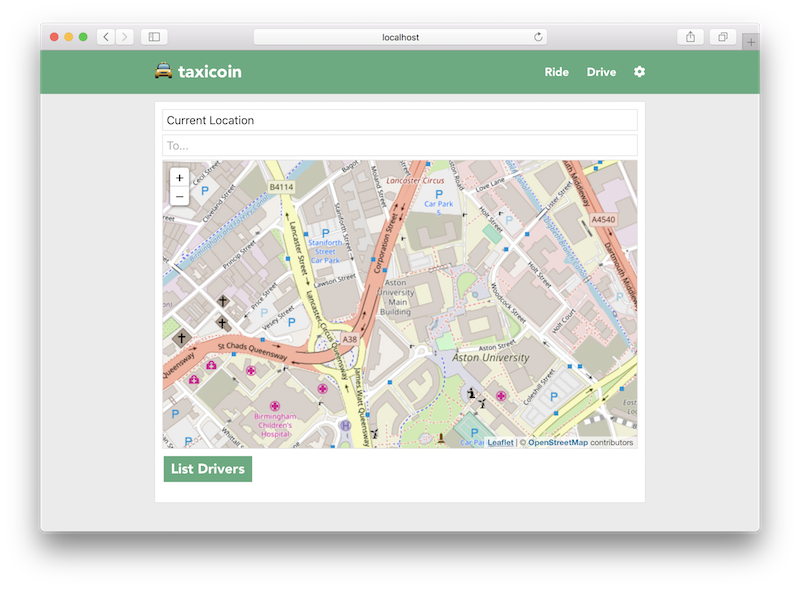
\includegraphics[width=12cm]{res/webapp.png}
\end{figure*}

Vue introduces the concept of \textit{reactive} data - when a JavaScript object changes value, any component which is using the data (observing it) automatically updates to use the new value. Retrieving the user's current location is a key requirement for any implementation of the Taxicoin protocol, and within a web browser this can be done using the geolocation browser API.

To adapt this for use with Vue's reactive models, a Vue \textit{plugin} has been created as part of this implementation. This creates a \lstinline{$location} object available to all components globally, which has latitude and longitude components, both of which are reactive.

Another plugin was also created for exposing a Taxicoin library instance to all components. This means that instead of needing to instantiate this for each page components and then pass it to child components where needed, the one instance is available globally.

Although this client implementation is functional, it is not feature complete at the time of writing, and does not implement all features of the library, such as sending of the driver's location to the rider, or a user interface for proposing a fare alteration. However, it is sufficient as a proof of concept.

Additionally, this application is most likely to be used from a mobile device (very few taxi drivers carry a laptop with them). This is possible using the Status mobile Ethereum browser \cite{Status.im}, which exposes a Web3.js object to web pages (also including Whisper protocol functionality, and in fact pioneering the 6th iteration of the protocol).

\pagebreak
\section{Verification and Validation}

As Taxicoin is intended to be a ubiquitous, maintenance-free, and open protocol, it is extremely important that implementations correctly conform to the standard, and that they are without issues. If, for example, one widely used implementation featured an incorrectly implemented method with unexpected side-effects, it could impact on the whole network of Taxicoin clients and contracts.

\subsection{Validation}

% Are we building the product right?
% Compare with protocol specification

In order to ensure this implementation of Taxicoin meets the protocol specification, various methods of validation have been used.

A series of functional integration tests validate the overall ability of the client library to interact with the smart contract instance, while conforming to the protocol specification.

Unit testing has also been performed on the smart contract itself to check the various pre- and post-conditions of each protocol method, as well as any additional internal methods not defined in the protocol.

Finally, a static analysis tool has been applied on the smart contract to check for common Solidity implementation errors.

\subsubsection{Functional Tests}

% Integration tests, based on protocol specification

The functional integration tests use the \textit{Ganache} \cite{Ganache} tool to emulate a blockchain, on which we deploy the Taxicoin contract. The framework used for testing is Mocha \cite{Mocha}, along with the Chai \cite{Chai} assertion library. The tests are orchestrated by Karma \cite{Karma}, which transpiles the JavaScript library and launches a Google Chrome browser instance in which to run the tests. Before each test, the state of the Taxicoin contract is reset, and a new Taxicoin library instance is constructed for use. These are then cleaned up in the after hook.

\begin{lstlisting}[language=JavaScript]
describe('driver accept journey', () => {
  it('should throw an error if the provided address (rider) has not agreed to ride with the driver', async () => {
    const riderAccount = await tcRider.getAccount()
    await expect(tcDriver.driverAcceptJourney(riderAccount)).to.be.rejected
  })

  it('should set the driver\'s state to being on a journey', async () => {
    const driverAccount = await tcDriver.getAccount()
    const riderAccount = await tcRider.getAccount()
    const fare = 100

    await tcDriver.driverAdvertise(51.5074, 0.1278)
    await tcRider.riderCreateJourney(driverAccount, fare)
    await tcDriver.driverAcceptJourney(riderAccount)

    const journey = await tcDriver.getJourney()
    journey.should.not.be.null
  })

  it('should remove the driver from the list of advertised drivers', async () => {
    const driverAccount = await tcDriver.getAccount()
    const riderAccount = await tcRider.getAccount()
    const fare = 8000

    await tcDriver.driverAdvertise(51.5074, 0.1278)
    await tcRider.riderCreateJourney(driverAccount, fare)
    await tcDriver.driverAcceptJourney(riderAccount)

    const drivers = await tcRider.getDrivers()

    expect(drivers).to.be.empty
  })
})
\end{lstlisting}


Each test group is based around one of the methods or messages, as described in the protocol specification. With the methods, we can easily construct each individual test scenario based on the pre- and post-conditions.

These tests ensure the technical requirements, as defined in the protocol specification, are met.

\subsubsection{Unit Tests}

% Unit tests on contract

As mentioned previously, Solidity is still a fairly immature language, however related tooling does exist for running unit tests. The Truffle framework \cite{Truffle} provides a Solidity-based testing tool, with standard assertions.

Unit tests have been used with Taxicoin to ensure that the contract (written in Solidity) performs the implemented functionality as expected. Each test case calls certain methods within the contract, given certain pre-conditions, and checks that the resulting state of the contract is as expected. An example test case is given below.

\begin{lstlisting}[language=Solidity]
contract TestTaxicoin {
  ...
  function testDriverAdvertise() public {
    Taxicoin tc = Taxicoin(DeployedAddresses.Taxicoin());

    string memory lat = "1.23";
    string memory lon = "50.67";
    string memory pubKey = "<pub_key_goes_here>";

    uint driverDeposit = tc.driverDeposit();
    tc.driverAdvertise.value(driverDeposit)(lat, lon, pubKey);

    FetchedDriver memory dr = getDriver(tc, tx.origin);

    Assert.equal(dr.addr, tx.origin, "driver addr should equal address of sender");
    Assert.equal(dr.lat, lat, "driver lat should equal advertised lat");
    Assert.equal(dr.lon, lon, "driver lon should equal advertised lon");
    Assert.equal(dr.pubKey, pubKey, "driver pubKey should equal advertised pubKey");
    Assert.equal(dr.updated, block.timestamp, "driver updated should equal block timestamp");
    Assert.equal(dr.deposit, driverDeposit, "driver deposit should equal global driver deposit");
  }
  ...
}
\end{lstlisting}

\subsubsection{Static Analysis}

% Using manticore

The Solidity static analysis tool \textit{Manticore} has been used to check for common Solidity programmer faults. This is done through a series of input generation for \enquote{inputs that trigger unique code paths}, as well as crash discovery of \enquote{inputs that crash programs via memory safety violations}.

Additionally, it is able to detect common unexpected cases such as integer overflow. As an example, if a contract featured some method for withdrawing funds and the amount to withdraw was calculated based on the addition user input, the user may be able to cause an overflow, and cause the amount to be withdrawn to be incorrect, resulting in a loss of funds.

This static analysis is yet another method for ensuring that the Taxicoin protocol can act entirely autonomously, without fault, in what should be assumed as a hostile environment.

\subsection{Verification}

% Are we building the right product?
% Compare with requirements

The above validation methods confirm that the technical specification for the project is met, however they do not provide a sense for whether the functional requirements of the project have been satisfied. The only way we can do this is to check each one individually.

Based on the below comparisons between functional requirements and implemented features, this implementation of the Taxicoin protocol satisfies all original core requirements, and also some of the additional requirements.

\subsubsection*{Drivers must be required to pay a deposit in order to advertise}

When advertising, if a driver does not provide funds of an amount greater than or equal to the contract-defined driver deposit value, then the contract will revert and throw an error. Therefore, this requirement is met.

\subsubsection*{Riders must advertise jobs to drivers on an individual basis}

An index of advertised drivers is available for all to see, including the public key of each, allowing a rider to send a \lstinline{Job Proposal} message via Whisper. There is no public listing of proposed jobs, and therefore rider privacy is not compromised. This meets the requirement.

\subsubsection*{The fare must be determined by quotes from driver}

When a driver receives a job proposal, they choose whether or not to accept it, and what fare they which to charge. This allows the driver to decide to adjust a fare based on the circumstances (e.g. congestion, distance). This requirement is met.

\subsubsection*{Riders must pay fares to a contract in advance}

When a rider formally creates a journey on-chain, they must provided at least the stated fare (plus deposit, see below) with the transaction or the transaction will fail. Additionally, when a driver then formally accepts the journey on-chain, they provided a value representing what they are expecting the fare to be, and if the rider's provided fare does not match, the transaction will fail. This is a security measure to prevent riders from tricking drivers. Both of these factors satisfy the requirement.

\subsubsection*{Riders must provide an additional deposit before starting a journey}

When formally creating a journey on-chain, a rider must provide funds greater than or equal to the stated fare (value passed as an argument), plus the contract-defined driver deposit, or the transaction will revert and throw an error. This meets the requirement.

\subsubsection*{Riders and drivers must both rate the other on completion of a journey}

The complete journey method requires a rating between 1 and 255 to be passed as an argument, or the method will not execute. Until this is called, both parties are unable to retrieve their deposits, and the driver is not paid their fare. This mutual stake ensures that it is in both party's interests to complete the journey with ratings. Therefore this requirement is met.

\subsubsection*{When a journey is completed, deposits should be returned to the respective parties, and the fare paid to the driver}

On the completion of a journey (once both parties have called the complete journey method), the deposits paid by either party are returned and the fare is paid to the driver. This satisfies the requirement.

\subsubsection*{Prospective drivers and riders should be able to informally communicate before forming a contract (additional requirement)}

This additional requirement was not implemented as it was not deemed essential, but would be in a future protocol revision.

\subsubsection*{Dispute resolution should be built into the system (additional requirement)}

If the driver and rider have a disagreement during the journey, they are able to propose a new fare to the other party, initiating a negotiation over the new fare, performed peer-to-peer via Whisper with \lstinline{Propose Fare Alteration} messages. When an agreement is met (both parties propose the same fare), the driver formally proposed the new fare on-chain, and the rider formally accepts it. If the new fare is higher, the rider must provide the difference with the transaction, otherwise the difference is returned to the rider.

Additionally, if the rider believes the driver has not provided the promised service, they may wish to entirely cancel the journey and pay have their fare returned. This can be achieved by setting a fare of zero. The journey may then be completed. This thoroughly meets the requirement.

\pagebreak
\section{Evalutation}

This final sections acts as an evaluation of the success of the Taxicoin project, both as a protocol and an implementation.

\subsection{Completeness of Requirements}

While Taxicoin does have defined behaviour for all perceived \enquote{normal} behaviours of drivers and riders, it is difficult to determine whether the requirements proposed in this document for a taxi protocol would satisfy all scenarios which could possibly be encountered when it is in use. However, for situations where it may not satisfy the needs, the protocol has been designed in such a way that it is almost always possible to recover from an unexpected situation.

For example, when a rider and a driver are participating in a journey, if for some reason it cannot be completed successfully, the fare for the journey can be adjusted (possibly to zero if this is desired) to account for such occurrences.

A potential flaw in the protocol is that if either party loses the ability to send transactions while a journey is in progress, neither will be able to end the journey and thus continue using the application. A solution to this would be enforcing time limits on responses from either party to ending a journey. If, after a certain period, no response has been received then the journey will be completed regardless with the assumption that the non-responsive party acted in the favour of the other (highest possible rating for example).

In terms of fairness, there is concern that a \enquote{will of the market} type approach of the reverse-bidding system implemented in the Taxicoin protocol will drive fares down to the point that they are no longer fair for the majority of drivers. However, more experienced drivers with higher reputation have basis on which to value their services more highly, and therefore can continue to charge higher fares.

A rider (and their client) is making a decision based on factors beyond just the cost of a journey when deciding which driver to accept. They also factor in the number of journeys a driver has completed previously, as well as their overall rating. This means that depending on the preference of the rider, they won't always accept the lowest possible fare.

Until the protocol is widely used, it is not possible to say whether this approach will be wholly successful. If it is not, the protocol can be altered to a more effective solution.

\subsection{Impact}

The premise of this entire project was that traditional taxi travel can be an unfair experience, and that riders and drivers are often at the mercy of large corporations, especially with more modern app-based services.

As far as taking the power away from a central authority goes, Taxicoin has achieved this by effectively utilising an Ethereum network based protocol, which doesn't place the trust of the service in any one participant's hands. In theory it should be nonsensical for one party to attempt to cheat the other, as they will lose their deposit, although the deposit must be significant enough for this mechanic to function correctly.

If a person wished to develop a Taxi app, their desired features should conceivably be possible to implement within the scope of a Taxicoin implementation. And in the case that this is not true, as the protocol specification is open source, they may submit proposed changes to it, or write an extension to it.

\subsubsection{Negotiation Standard}

Taxicoin uses its own novel method of negotiation, where two parties first agree on a price for a service off-chain (through Whisper), and then make a formal agreement on chain. This is a method which may potentially be used with a myriad of other applications.

As such, it would be sensible for a generic standard to be developed for this purpose. This would allow for the development of other contracts which can participate in negotiations which follow the standard, in a similar way to, for example, interfaces in programming languages which support polymorphism.

\subsection{Future Development}

There is certainly room for improvement in both the protocol, and the implementation presented in this document.

\subsubsection{Additional Features}

There are several mentions throughout this report of potential improvements to the protocol. One such is the inclusion of a message type for informal \enquote{chat} between rider and driver before and during a journey. Although the protocol functions without this, it would be useful to be able to communicate special requirements, for example.

The Taxicoin JavaScript library makes heavy use of the \textit{Web3.js} library and signing transactions on a local Ethereum node, which functions adequately, but can be inflexible. If the user does not have access to their own local node, they may wish to use a third party node, such as the Infura service \cite{Infura}. In order for this to be secure, a user's signing key must not be transmitted to the third party. Therefore, a reasonable improvement to allow this would be to implement the signing of transactions locally (from JavaScript). This can be achieved either with Web3, or via an alternative such as \textit{Ethers.js}.

Additionally, due to the interaction-based nature of the protocol, there are likely to be some \enquote{rough edges} around the protocol, for which certain aspects will have to be adjusted. These are most likely to be focused around unforeseen exceptional circumstances.

As the protocol has been designed around an open ecosystem of independent implementations, it is hoped that such implementations will begin to be written. The core of these will likely be interaction libraries for various languages (other than JavaScript), and indeed one such library is already under development for the Go language \cite{TaxicoinGo}, based on the protocol specification in this document.

\subsubsection{Licensing Considerations}

At present, taxi drivers are required to hold a license in order to operate in many areas. In it's current state, the Taxicoin protocol could potentially support checking whether a driver is allowed to operate. However, this would require a blockchain-based \textit{oracle}, maintained by the body which issues taxi licenses. This would allow other smart contracts on the network to view the records of drivers (the issuing body would also have to publish an identifying address of the driver).

From a technical point of view, this is a very simple step to take. However, it would likely be blocked by local government bureaucracy, therefore it is not feasible at current, and it was not included in the project for this reason.

Identity on blockchain-based networks is still a relatively new topic. Many research projects are targeting the issue, therefore it is hoped that an agreed-upon solution and standard will be available in the near future.

\subsubsection{Client Algorithms}

The specification states that certain decisions are intended to be made in a semi-autonomous way. This includes the fare negotiation stage when a rider proposes a job to a set of drivers.

In the naive example client presented previously, the rider and driver fare negotiation is a manual process, however in reality it should function somewhat like the following: the driver's client determines an initial fare based on distance of journey and any other parameters. The rider's client then either approves or rejects, based on its threshold of what it believes a fair price to be. In the case of a rejection, the driver's client would incrementally decrease the fare quote until a threshold set by the driver is met, at which point the driver's client would reject the job.

There are many factors to be considered when developing this algorithm, thus why it was out of the scope of this project.

\section{Conclusion}

The Taxicoin protocol provides a strong basis on which developers can build taxi hailing applications which can be freely extended and allow for interoperability.

As a user of an application which implements Taxicoin, riders can expect a uniform straightforward experience, where fares are decided by quotes from multiple drivers. Instead of the cost of a journey being dictated by a central authority, they receive the best possible fare available to them.

As a driver, in contrast to other taxi applications, users receive fares in their entirety. This allows them to both charge less in order to be a more compelling option to competitors, and earn more.

In the context of fairness, Taxicoin should create an environment where all parties involved cannot have conditions forced upon them, nor be cheated. The protocol specification and implementation successfully achieve this, and it is hoped that the protocol will be built upon and implemented in a variety of future applications.

\pagebreak

\printbibliography[heading=bibintoc]
\pagebreak

\section*{Appendix}
\addcontentsline{toc}{section}{Appendix}

\subsection*{Project Diary}
\addcontentsline{toc}{subsection}{Project Diary}

The following in-person formal meetings were held. In addition to these, there was much discussion via email.

\begin{description}
    \item [3rd October 2017] talked about the fact that this project is relevant to the interests of the ALICE group. It is effectively a self-governing application. Was decided that the focus should be on compiling a list of ``must have'' features and then implementing them.
    \item [16th October 2017] was suggested to write a RFC-style protocol specification, to be used later to test against to determine if the implementation is correct.
    \item [13th November 2017] no huge amount of progress was reported due to other commitments. We revisited the idea of producing an RFC-style document, focusing on the IMAP protocol as an example.
    \item [4th December 2017] we discussed that including a network architecture diagram in the report would be a good idea of explaining how various parts of the project communicate with each other (e.g. front end talks to contract, different instances of front end talk to each other). At this point, a working implementation had been completed, therefore we began talking about how to write tests. It was decided that the contract should be tested directly with unit tests, and potentially integration testing performed on the Javascript abstraction layer and contract. We discussed that it would be good to get to the point where the application could be security audited.
    \item [14th Feburary 2018] in-person meeting was cancelled. Via email we discussed opportunities for research into the Ethereum field at the ETHDenver event which I was to attend. The RFC concept was developed further into a comprehensive protocol specification.
    \item [16th April 2018] Feedback was given based on the the current state of the report. It was suggested that the protocol definition section be altered to be \enquote{more formal}, and an example was given of what this may look like. The key part of this was the addition of pre- and post-conditions to each method. Additionally, it was suggested that all protocol method definitions share an identical format to make it easier to understand from a technical point of view. What was the \enquote{testing} section was recommended to be renamed to \enquote{verification and validation}.
\end{description}

\pagebreak
\subsection*{Project Readme}
\addcontentsline{toc}{subsection}{Project Readme}

Taxicoin is a decentralised ride-sharing protocol, which uses Ethereum to manage logistics. The aim of the project is to provide a more open alternative to existing applications, and one without any intermediary to take a cut of driver profits.

It is the final year project of Scott Street, a Computer Science undergraduate at Aston University, Birmingham. As such, please do not attempt to contribute!

\subsubsection*{Running Locally}

You'll first need to install the project dependencies: \lstinline{nodejs}, \lstinline{npm}, \lstinline{ganache}, \lstinline{geth}.

\medskip

1. Clone this repo to somewhere on your computer

2. Launch `ganache`, make sure it's using port `7545` and leave it running in the background

3. Run `geth` using the following, and keep it running in the background:

\begin{lstlisting}
# run on rinkeby testnet, allow anybody to connect, and enable the Whisper protocol
geth console --rinkeby --rpc --rpccorsdomain "http://localhost:*" --shh
\end{lstlisting}

4. Run some commands to set everything up:

\begin{lstlisting}
cd /where/you/put/taxicoin
# install dependencies
npm install
# migrate Ethereum smart contracts
npm run contract
# start the dev server
npm run dev
\end{lstlisting}

5. This should open a browser window at `http://localhost:8080` where you can start playing with Taxicoin!

\subsubsection*{Multiple Accounts for Testing}

As a single user of Taxicoin is not able to be both a rider and a driver simultaneously, for testing purposes it is useful to be able to use two Ethereum accounts. The browser plugin \lstinline{MetaMask} allows this.

After installation, set the network to custom RPC, with the url \texttt{http://127.0.0.1:7545} (your local ganache test node). In ganache, you may click the key icon to the right of each address to display the private key for that address. You may then use this to import the account into MetaMask.

Now when visiting the Taxicoin example client, it will automatically use MetaMask to interact with the smart contract. Simply toggle between two imported Ganache accounts to represent either a rider or driver.


\subsection*{Code Listings}
\addcontentsline{toc}{subsection}{Code Listings}

The code listings have not been included to save printing. However, the full source code may be found attached, or alternatively is freely available under the MIT software license at \url{https://github.com/sprusr/taxicoin/}.

%\subsubsection*{Taxicoin Contract}
%\addcontentsline{toc}{subsubsection}{Taxicoin Contract}
%
%\lstinputlisting[language=Solidity]{../contracts/Taxicoin.sol}
%
%\subsubsection*{Taxicoin JavaScript Client Library}
%\addcontentsline{toc}{subsubsection}{Taxicoin JavaScript Client Library}
%
%\lstinputlisting[language=JavaScript]{../src/script/taxicoin.js}

\pagebreak
\subsection*{Project Definition}
\addcontentsline{toc}{subsection}{Project Definition}

\subsubsection*{Subject}

When the Internet was in its infancy, if you wanted to use it for a specific application, you might have written a protocol. That way, anybody who wanted use the Internet for that purpose would have a common way of doing it - and if a new person came along and wanted to join in, they could just write their software to conform with the standard.

In the past 15-or-so years however, the landscape has changed. Companies now favour their own proprietary systems, where they can have complete control, and ultimately gain the most profits. Specifically companies such as Uber have taken an industry which was once fairly well distributed, and put the control in their own hands - they decide who can be a driver, they manage the fares, and how much they pay their drivers.

But recent developments with distributed networks threaten to disrupt this comfy business model. Technologies such as Ethereum allow "trustless" applications, where activities of a single node are verified by the entire network. It's an area which is yet to be explored to its full potential, but all the features needed to be able to implement feature-rich apps are there. The logic of applications running on such a system has to be rethought, but with Uber as an example, there would be no central authority to take a cut of profits. The entire system would be self-regulating.

\subsubsection*{Deliverable}

A ride-sharing webapp accessible with an Ethereum network-enabled browser, designed in such a way that no single entity has control over the running of the system. Drivers will be able to advertise their location (published to blockchain), and riders will be able to send job proposals (containing pickup and drop-off locations) to these drivers on a peer-to-peer basis. This protects the privacy of the rider by ensuring that only the chosen drivers are able to see the rider’s location. When a driver initially advertises their location, they are required to provide a deposit to the network, which will be returned in completion of a trip. This gives the driver a stake in wanting to complete a journey, and should reduce spam on the network.

Drivers are then able to issue a response to a proposal, by either rejecting or quoting a price for the journey. This allows drivers to choose which journeys they take, and prevents drivers from having to travel a long distance to a pickup location, compared with if the allocation was done randomly. Should the rider choose to accept the quote, then both rider and driver form an agreement via a smart contract on the Ethereum network. This includes the passenger offering up the cost of the journey, plus an additional deposit equal to the amount the driver provided previously.

At this point, the fare for the journey, a deposit from the rider, and a deposit from the driver are all held by a smart contract. This acts as an incentive for the driver and rider to successfully complete the physical journey. When this is done, and both parties are in agreement that it is completed, then the deposits can be returned and the fare paid to the driver.

All monetary transactions will be executed with cryptocurrency on the Ethereum network, so as to minimise fees and prevent the transaction from being intercepted by a third party.

As the vast majority of interactions between riders and drivers will be based on no existing knowledge of the other party, a reputation system will be used to form a layer of trust. Based on previous journeys, and the ratings given to both rider and driver on completion of each, future riders will be able to make informed decisions about which drivers to send job proposals. And in the same fashion, drivers will be able to decide which riders’ proposals to accept.

\subsubsection*{Originality}

Although ride-sharing apps aren’t a new thing, nearly all existing solutions are controlled by a central authority who take a cut of the profits. This means users are at the mercy of the company when it comes to fares, and drivers must be approved, potentially opening the way for discrimination.

This project eliminates these problems by taking control away from any one part of the system. All transactions take place in a peer to peer nature, with the network being the only intermediary. This ensures that the two parties involved have full control over the process, whilst at the same time preventing one from cheating the other.

\subsubsection*{Timetable}

The following proposed timetable will be used to track progress over the course of the project. The work is broken down into fortnightly blocks. Through the entirety, a project diary will be kept to keep track of key decisions. This is to be used as the basis for much of the final report.

\begin{center}
  \begin{tabularx}{0.85\textwidth}{ |l|X| }
    \hline
    Date & Planned Activity \\ \hline
    02/10/17 & Begin writing a formal project definition. Decide on project objectives, and have an idea of what features will be included. Which features would the system not work without. \\
    \hline
    16/10/17 & Finish project definition. Begin mapping out interactions of users with the system and other users as a diagram. Create protocol documentation - similar to RFC. This is to be used to test against.
    \textbf{Project definition due 20th October} \\
    \hline
    30/10/17 & Start implementing said protocol, with aim of creating fully function implementation (not including user interface). Test against RFC-style document. \\
    \hline
    13/11/17 & Finish initial protocol implementation. \\
    \hline
    27/11/17 & Develop testing suite for protocol implementation. \\
    \hline
    11/12/17 & Fix any issues with implementation, and complete testing. Begin TP1 progress report. \\
    \hline
    25/12/17 & Continue TP1 progress report. \\
    \hline
    08/01/18 & Exams scheduled in this period, therefore expecing a slow down in project work.
    \textbf{TP1 progress report due 19th January.} \\
    \hline
    22/01/18 & Continuation of development based on progress report. Begin writing of final report. \\
    \hline
    05/02/18 & Research into how to develop the user interface. Review of existing mobile Ethereum clients. \\
    \hline
    19/02/18 & Development of user interface. \\
    \hline
    05/03/18 & Addition of identified "stretch" features. \\
    \hline
    19/03/18 & Finalising development and report writing. \\
    \hline
    02/04/18 & Report writing. \\
    \hline
    16/04/18 & Finalising report and considering how to present the project during demos.
    \textbf{Final submission due 27th April.} \\
    \hline
  \end{tabularx}
\end{center}

\pagebreak
\input{tex/appendix/tp1-progress-review}

\end{document}
